\documentclass[../../main.tex]{subfiles}

\graphicspath{{../../fig/}}
\setcounter{section}{0}

\begin{document}

\chapter{ワイヤーのたわみ量評価系の開発と、自動化手法の確立}
\label{chap:wiresag}
較正に使う直線偏光はワイヤーに沿う形で生成されるため、ワイヤーがたわんでいる部分から生成される光はその偏光角が
ワイヤーに沿う方向からずれて生成される。そのため、ワイヤーのたわみは較正の精度に影響を及ぼし、系統誤差を生む。
\ref{subsec:wg_wiresag}項では、過去に行われた評価手法について述べ、この手法にはいくつかの問題があった。
本章では、初めにこの問題について今一度触れたあと、それを解決するために開発したワイヤーのたわみを評価する系について述べる。
その後、評価系の性能評価を行い、最後に実際にスパースワイヤーグリッドに対して行った評価結果について述べる。

\section{過去の測定手法における問題点と開発目標}
\colortext{blue}{過去の測定手法についてもう一度 review するべきか、
それとも\ref{subsec:wg_wiresag}項をもっと簡素にし、詳細な内容をこちらに持ってくるべきか、
現在のようにrefするだけにするべきか悩んでいる。}

過去の測定手法については\ref{subsec:wg_wiresag}項にて述べたとおりであり、その手法にはいくつかの問題点があった。
一つ目の問題点は、その測定精度が低いことである。これはたわみ量の系統誤差への寄与を必要以上に大きくしている。
また、図\ref{fig:wiresag_result_old}にて示されているように、
全てのワイヤーに対してそのたわみ量は期待される量からどの程度外れているかを判別できておらず、
品質の低いワイヤーを選別できていない。
もう一つの問題点は、その測定手法が人力にて行われており、測定のために労力と時間がかかる点である。
これによりスパースワイヤーグリッドの量産、品質の保証・管理のために繰り返し測定することが困難である。
また、人力での測定はその測定結果に人依存のバイアスを産む可能性がある。

以上の問題点を解決するため、
\begin{enumerate}
    \item ワイヤーのたわみ量を $\order{\SI{10}{\mu m}}$ の精度で評価可能であること
    \item 全てのワイヤーのたわみ量を自動的に評価可能であること
\end{enumerate}
という2点の開発目標をもって新たなワイヤーのたわみ量の評価系を開発した。

\section{評価系の概要と評価原理}
\subsection{評価系の概要}
初めに、作成した評価系の概観を図\ref{fig:wiresag_system}に示す。
基本的な評価原理は\ref{subsec:wg_wiresag}項にて述べた過去の手法と同様であり、
ストレートエッジとワイヤーを同一写真内に映るように撮影することで、ストレートエッジとワイヤー間の距離からワイヤーのたわみを評価する。
より高精度な評価と自動化を実現するため、過去の評価系をもとに以下の変更を行った。
\begin{enumerate}
    \item スパースワイヤーグリッドを鉛直方向に立てて撮影を行う
    \item スパースワイヤーグリッドとカメラをアクチュエータを用いて自動的に動かす
    \item 一つのワイヤーに対して両端と中央だけでなく、複数の点で撮影を行う
\end{enumerate}

アクチュエータによる自動化を容易にするため、スパースワイヤーグリッドを鉛直方向に立てる。
たわみの測定の基準となるストレートエッジはスパースワイヤーグリッドの目の前 $\SI{5}{mm}$ のところに固定されている。
自動化の要であるアクチュエータは、スパースワイヤーグリッドを鉛直方向に動かすために Openbuilds 社の V-Slot NEMA 23 Linear Actuator (Belt Driven) を、
カメラを水平方向に動かすために Openbuilds 社の V-Slot NEMA 17 Linear Actuator (Belt Driven) を用いた。
どちらもベルト駆動式であり、ステッピングモーターを用いて位置制御を行うことができる。
スパースワイヤーグリッドに取り付けられたアクチュエータは、ストレートエッジとワイヤーの距離をカメラの画角に収まるように近づけるために使用され、
カメラに取り付けられたアクチュエータは、撮影位置を変え、ストレートエッジとワイヤーの距離を複数の点で測定するために使用される。
アクチュエータの制御には、Galil 社の DMC-4020 というモーションコントローラを用いた。

\begin{figure}[H]
    \centering
    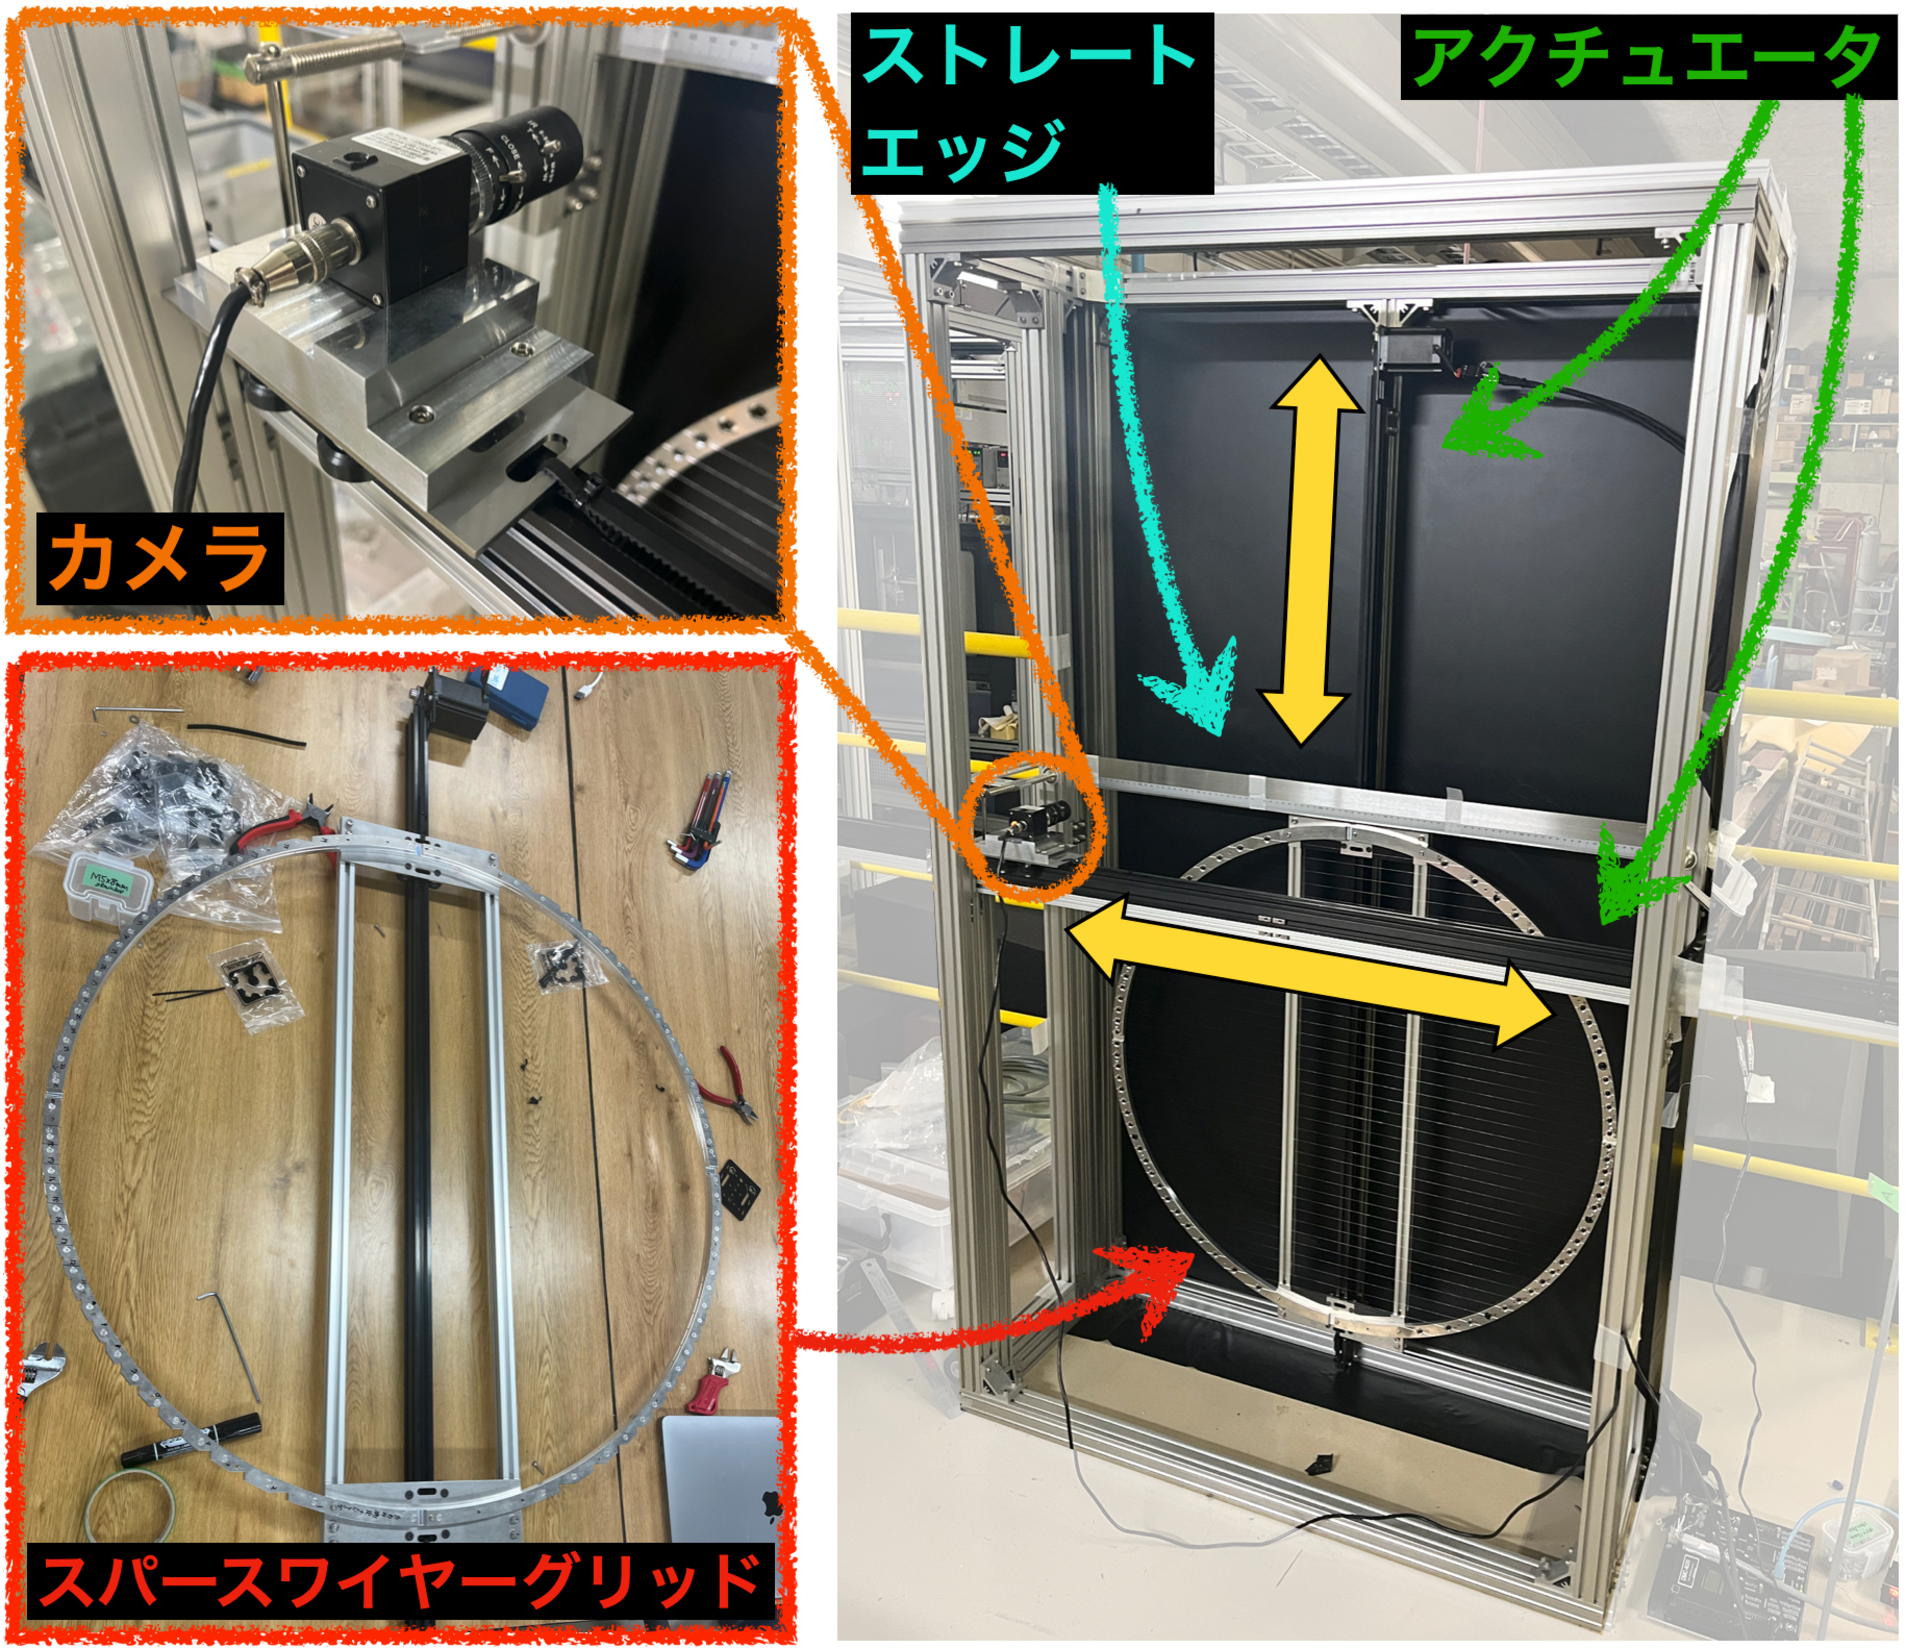
\includegraphics[width=0.8\textwidth]{wiresag/wiresag_system.pdf}
    \caption{ワイヤーのたわみ量評価系の概観}
    \label{fig:wiresag_system}
\end{figure}

\subsection{評価原理}
図\ref{fig:wiresag_concept}に評価原理の概念図を示す。
$x_{0},\,x_{1},\,\cdots,\,x_{n}$ は撮影箇所の位置を表し、$z_{0},\,z_{1},\,\cdots,\,z_{n}$ は各写真から測定されるストレートエッジとワイヤーの距離である。
得られた $x_{i},\,z_{i}$ を横軸 $x$、縦軸 $z$ でプロットすると、ワイヤーの概形を表す曲線が得られる。
ワイヤーの理論曲線はワイヤーの素材、かかっている張力により決まるカテナリー曲線であるため、
得られた曲線をカテナリー曲線で fitting することでワイヤーのたわみ量を評価することができる。

ワイヤーの概形を表すカテナリー曲線は、$T$ をワイヤーにかかる張力、$\rho_{\mathrm{W}}$ をワイヤーの密度、
$R_{\mathrm{W}}$ をワイヤーの半径、$L_{\mathrm{frame}}$ をワイヤーを固定している両端間の距離として
\begin{align}
    f(x;a) &= a\cosh\qty(\dfrac{x+L_{\mathrm{frame}}/2}{a}) - a\cosh\qty(\dfrac{L_{\mathrm{frame}}}{2a}) \\
    a &= \dfrac{T}{\rho_{\mathrm{W}}\cdot\pi R_{\mathrm{W}}^2}
\end{align}
と表される。なお、この式は原点 $(0,\,0)$ と $(L_{\mathrm{frame}},\,0)$ を通る拘束条件を課したカテナリー曲線を表している。
スパースワイヤーグリッドにはタングステン製のワイヤーを使うため、その密度は $\rho_{\mathrm{W}}=\SI{19.3}{g/cm^3}$ であり、
ワイヤーの半径は $R_{\mathrm{W}}=\SI{0.1}{mm}$ である。
$L_{\mathrm{frame}}$ はどのワイヤーを評価するかによって異なる。
図\ref{fig:wire_number}のようにスパースワイヤーグリッドに張られたワイヤーに通し番号をつけたとき、
スパースワイヤーグリッドの内径が $\SI{790}{mm}$ であり、ワイヤー間のピッチが $\SI{20}{mm}$ であることから、
$n$ 番目のワイヤーにおける $L_{\mathrm{frame}}$ は
\begin{align}
    L_{\mathrm{frame}, n} = 2\sqrt{395^2-(20\cdot(19-n))^2}\ [\mathrm{mm}] \quad (n=1,2,\cdots,19)
\end{align}
と表される。

\begin{figure}[H]
    \centering
    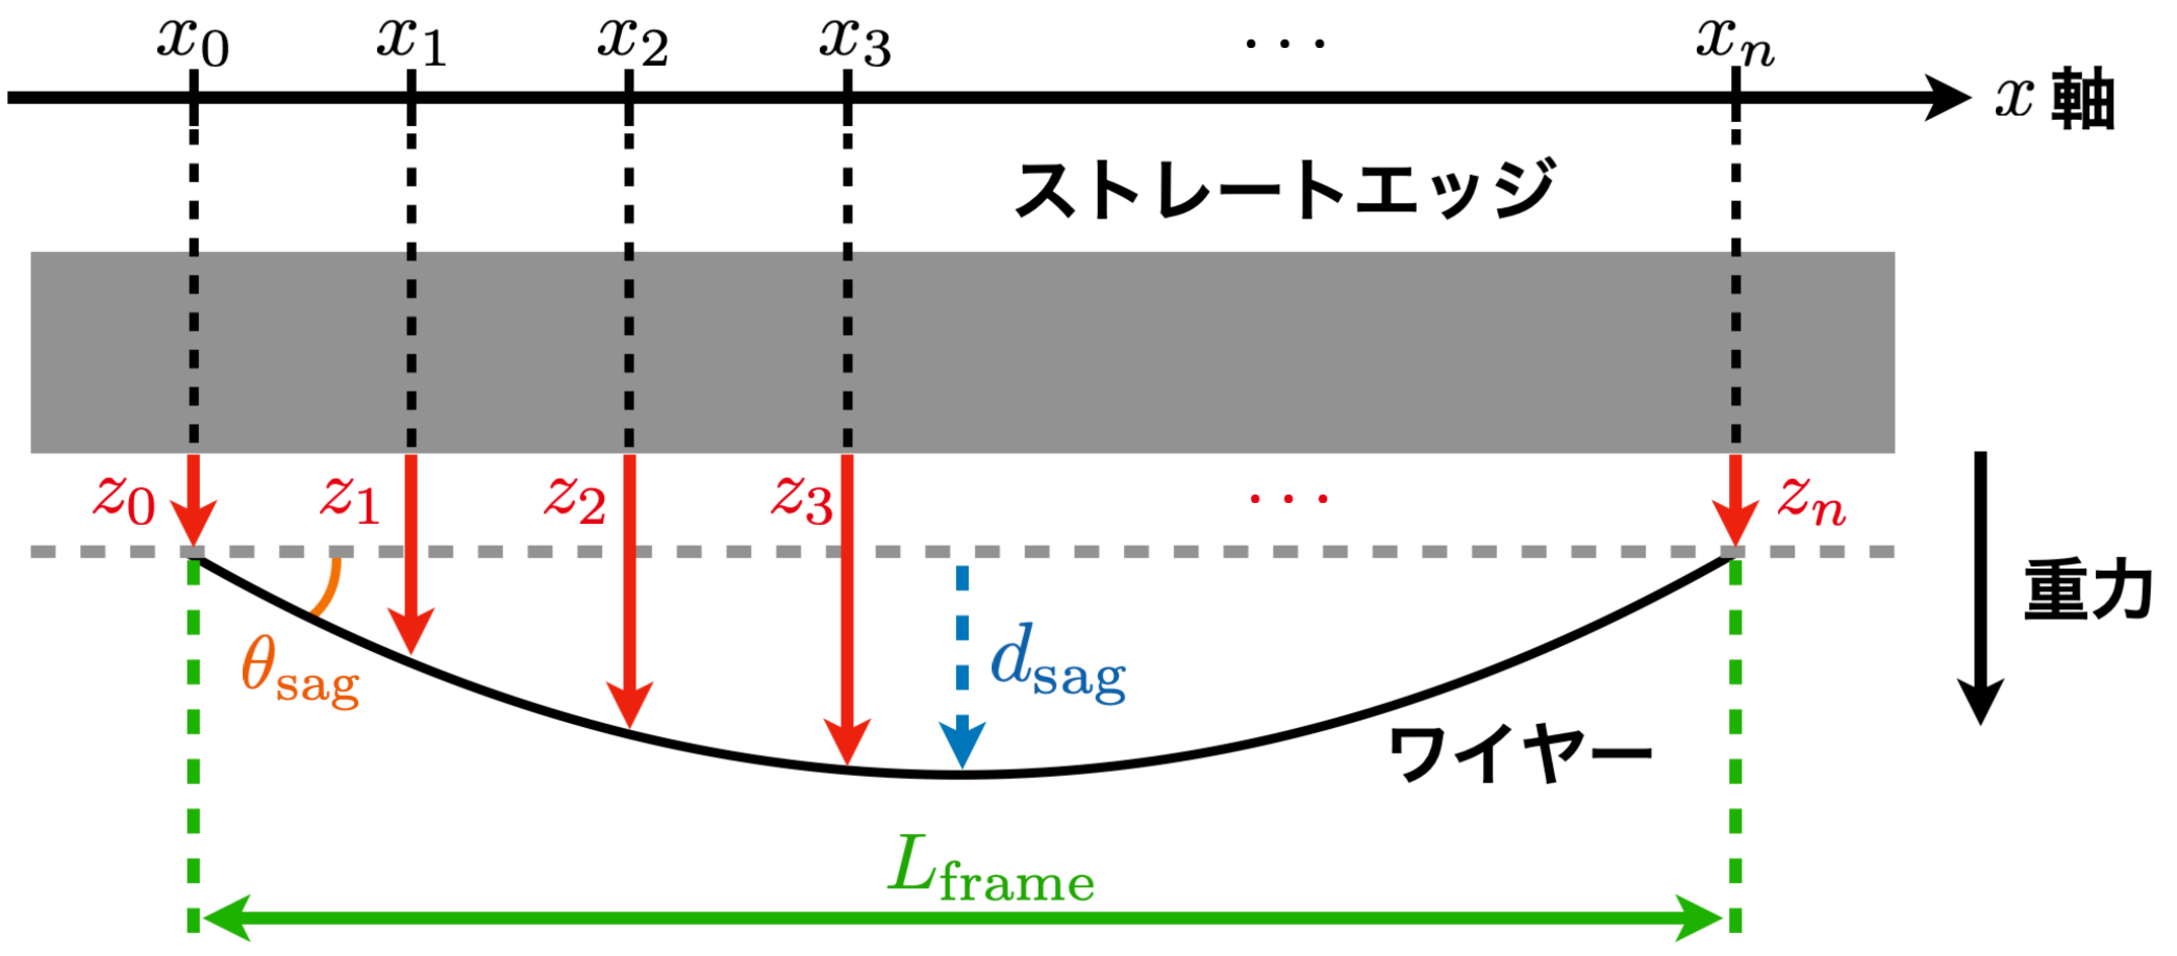
\includegraphics[width=0.8\textwidth]{wiresag/wiresag_concept.pdf}
    \caption{ワイヤーのたわみ量の評価原理}
    \label{fig:wiresag_concept}
\end{figure}
\begin{figure}[H]
    \centering
    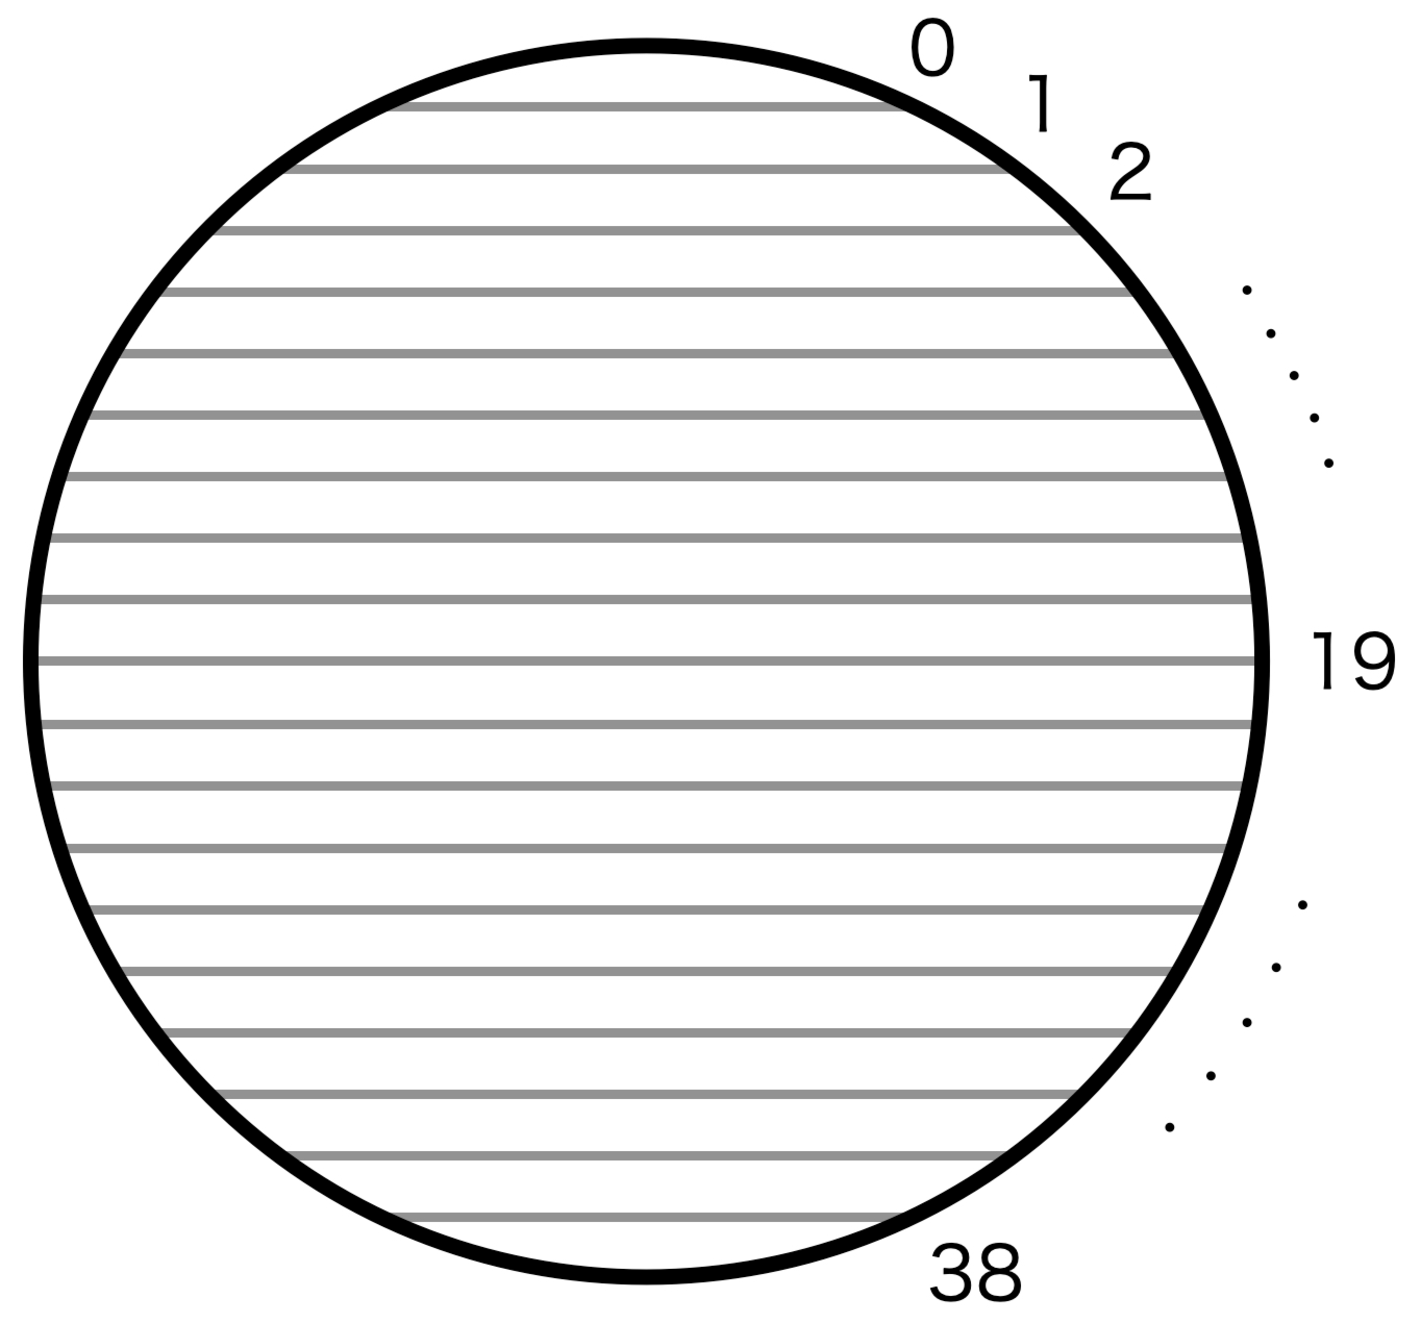
\includegraphics[width=0.5\textwidth]{wiresag/wire_number.pdf}
    \caption{スパースワイヤーグリッドにおけるワイヤー番号}
    \label{fig:wire_number}
\end{figure}

図\ref{fig:wiresag_concept_yoko}にワイヤーのたわみ量の評価原理の横から見た概念図を示す。
これは過去の手法における概念図\ref{fig:wiresag_setup_old}を新しい系に合わせて変更したものであり、
カメラから見るとストレートエッジが手前に位置し、ワイヤーがその奥に位置するような配置になっている。
各パラメータの意味とその値を表\ref{}に示す。
この系において、測定される量 $z'$ を用いてストレートエッジとワイヤー間の距離 $z$ を表すと、
\begin{align}
    z = \dfrac{z'}{\cos\phi} + \alpha\tan\phi \\
    \phi = \arctan\qty(\dfrac{L_{\mathrm{camera}}}{\beta})
\end{align}
となる。
過去の手法における誤差の主原因として、$\phi$ が典型的に $5\tcdegree$ 程度と小さくない値であったために、
$L_{\mathrm{camera}}$ や $\alpha$ から $z$ へ大きな誤差が生じていたことが挙げられる\cite{swg:murata}。
過去の評価系において $\phi\sim0$ すなわち $L_{\mathrm{camera}} \sim 0\tcdegree$ で撮影ができていなかった理由は、
スパースワイヤーグリッドを水平面上に設置して撮影しており、他のワイヤーが撮影対象のワイヤーに重なってしまうためである。(図\ref{fig:wiresag_picture_old})
これを解決するため、スパースワイヤーグリッドを鉛直方向に立てて撮影を行うことで、$L_{\mathrm{camera}}=0\pm\SI{0.5}{mm}$ で撮影を行い、誤差の低減を図った。
\begin{figure}[H]
    \centering
    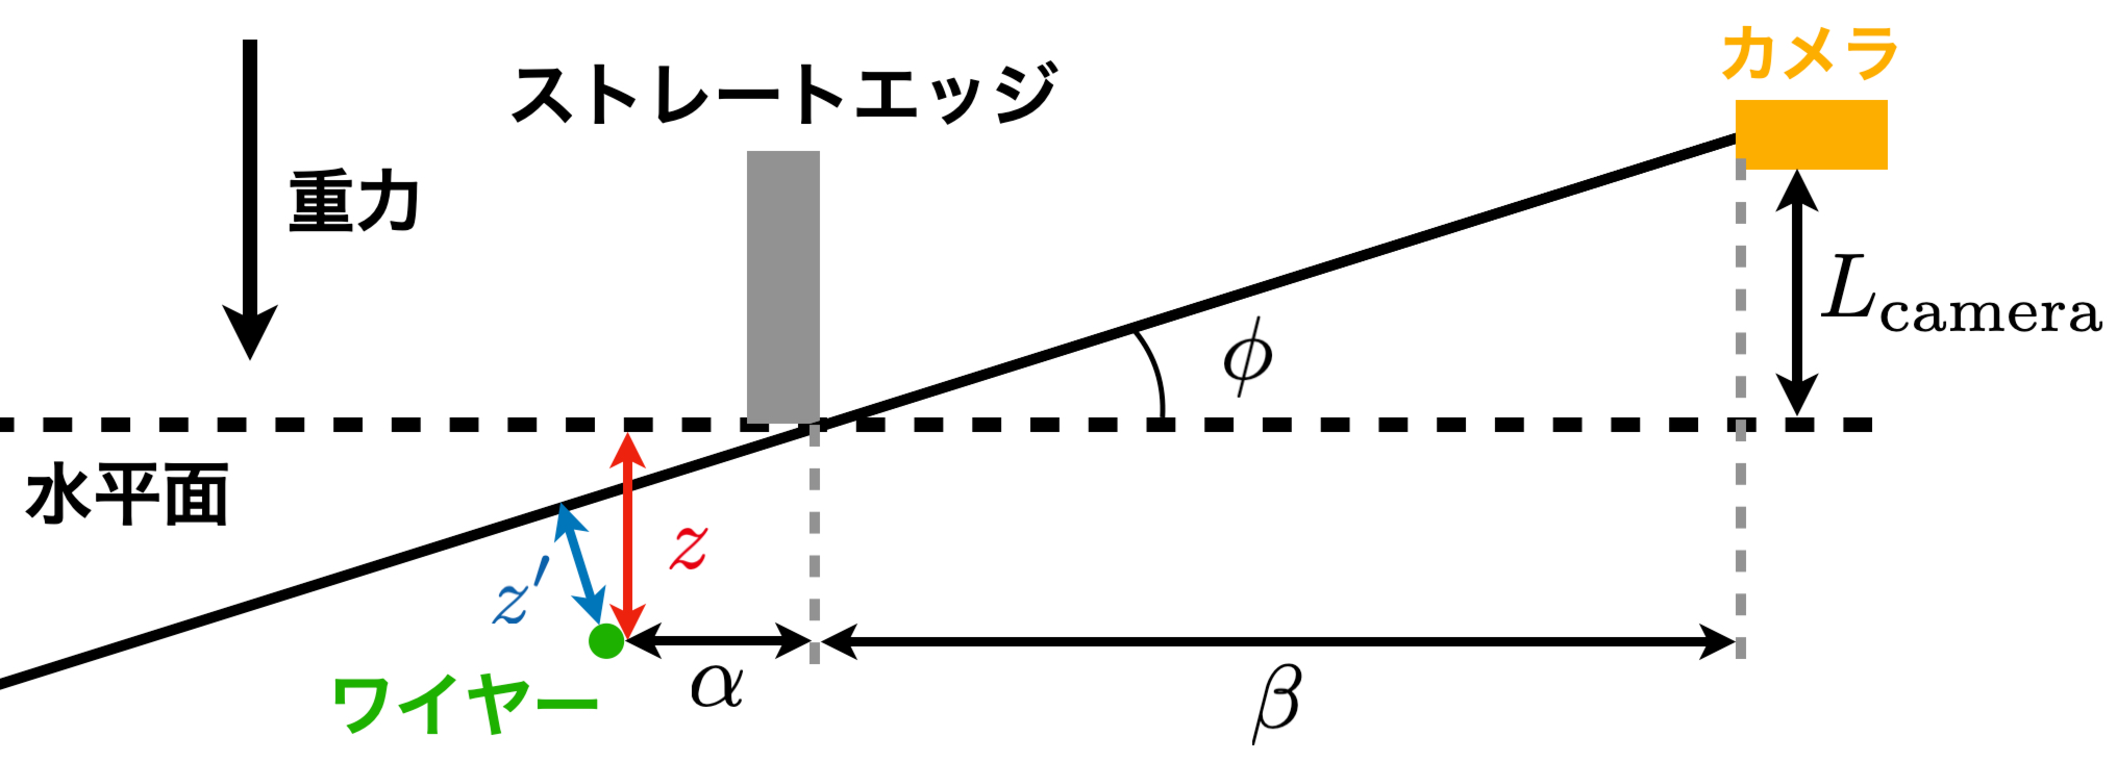
\includegraphics[width=0.8\textwidth]{wiresag/wiresag_concept_yoko.pdf}
    \caption{ワイヤーのたわみ量の評価原理の横から見た概念図}
    \label{fig:wiresag_concept_yoko}
\end{figure}
\begin{table}[H]
    \centering
    \caption{図\ref{}における各パラメータの意味と値}
    \begin{tabular}{cccc}
        パラメータ & 意味 & 値 & 誤差 \\
        \hline\hline
        $\alpha$ & ストレートエッジとワイヤーまでの水平距離 & $\SI{15}{mm}$ & $\pm\SI{2}{mm}$ \\
        $\beta$ & ストレートエッジからカメラまでの水平距離 & $\SI{205}{\mm}$ & $\pm\SI{5}{mm}$ \\
        $L_{\mathrm{camera}}$ & ストレートエッジ下端の面からカメラまでの鉛直距離 & $\SI{0}{mm}$ & $\pm\SI{0.5}{mm}$ \\
    \end{tabular}
\end{table}


\section{解析手法}

\section{開発した評価系の原理検証}
\subsection{評価手法}
\subsection{評価結果とその考察}

\section{スパースワイヤーグリッドのたわみ量の評価}

\end{document}